\documentclass[11pt]{article}

\usepackage[margin=1in]{geometry}
\usepackage{amsmath,amssymb}
\usepackage{booktabs,tabularx,array}
\usepackage{graphicx}
\usepackage{xcolor}
\usepackage{microtype}
\usepackage{enumitem}
\usepackage{caption}
\usepackage{subcaption}
\usepackage{float}
\usepackage{placeins}
\usepackage{fancyhdr}
\usepackage[hidelinks]{hyperref}

\definecolor{ink}{HTML}{263238}
\definecolor{blue}{HTML}{1F4E79}
\definecolor{lightblue}{HTML}{EAF1F7}
\definecolor{rulegray}{HTML}{CBD3D9}
\definecolor{muted}{HTML}{5F6B73}

\hypersetup{
  colorlinks=true,
  linkcolor=blue,
  citecolor=blue,
  urlcolor=blue
}

\captionsetup{font=small,labelfont=bf}
\setlist{nosep,leftmargin=1.6em}
\setlength{\parindent}{0pt}
\setlength{\parskip}{0.55em}
\renewcommand{\arraystretch}{1.14}
\pagestyle{fancy}
\fancyhf{}
\fancyhead[L]{\small Global RBF collocation}
\fancyhead[R]{\small Classical and recycle-space study}
\fancyfoot[C]{\thepage}
\setlength{\headheight}{14pt}

\newcommand{\R}{\mathbb{R}}
\newcommand{\norm}[1]{\left\lVert #1\right\rVert}
\newcommand{\trans}{^{T}}
\newcolumntype{Y}{>{\raggedright\arraybackslash}X}

\title{\textbf{Global RBF Collocation and Difficult-Space Recycling}\\
\large A validated progression from dense classical solvers to transfer diagnostics}
\author{Global RBF Collocation Research Branch}
\date{September 5, 2026}

\begin{document}

\maketitle

\begin{abstract}
This report consolidates the complete global radial basis function collocation study. The central question is whether a strong classical preconditioner leaves a small, reproducible difficult space that can be reused or learned. The discretization is correct on the resolved native-basis path. Dense FP64 LU is fastest at moderate size, FP32 pivoted LU is the strongest reusable iterative baseline for the $N=225$ families, and an RBF-specific local least-squares approximate-cardinal factor becomes useful only in selected regimes. Several system-own oracle spaces reduce iterations, but their value depends sharply on how the coarse space is integrated into FGMRES. A harmonic-Ritz recycle space gives a clear 27.6\% reduction on one deliberately difficult $N=400$ problem, yet adjacent shape-parameter transfer has median iteration ratio near one. Cluster-aware ranks do not repair the failure. Normalized residual-history POD is neither persistent nor geometrically stable. An offline data set was built, but its shared basis needs 158 of 225 ambient directions and its oracle target does not improve the aggregate solver. The present evidence therefore supports continued numerical target design, not neural training.
\end{abstract}

\section{Research framework}

The algorithmic program begins with the dense global collocation matrix rather than with assumptions imported from sparse RBF-FD. Its full logic is:

\begin{enumerate}[label=\textbf{\arabic*.}]
  \item Assemble and verify the native global RBF discretization for a manufactured elliptic problem.
  \item Measure conditioning, density, memory, and true-residual convergence while separating discretization failure from solver difficulty.
  \item Compare dense and RBF-specific classical preconditioners, then select a primary action $M^{-1}$.
  \item Characterize the unresolved inverse action and define candidate difficult spaces from singular vectors, correction snapshots, residual histories, and Krylov data.
  \item Test each exact space with a mathematically matched coarse or projected-Arnoldi integration. Random spaces and the classical solver remain controls.
  \item Vary one system parameter at a time and compare within-system numerical variability with between-system subspace motion.
  \item Reuse and interpolate spaces before considering prediction. Solver iterations and true residuals decide usefulness, not projector error alone.
  \item Build a learning data set only after an oracle target is useful, low dimensional, and stable enough to justify prediction.
\end{enumerate}

The study repeatedly returned to an earlier step when a later diagnostic failed. This is important because the final outcome is not a sequence of independent stage conclusions. It is one narrowing argument. Global collocation admits strong same-system oracles, but the useful directions are highly coupled to the operator, the preconditioner, the right-hand side, and the augmentation formula.

\section{Numerical formulation and solver machinery}

The domain is $\Omega=[0,1]^2$. Most experiments use the Poisson problem $-\Delta u=f$ with homogeneous Dirichlet data and manufactured solution $u(x,y)=\sin(\pi x)\sin(\pi y)$. The parameterized diffusion family uses $-\nabla\cdot(a_\beta\nabla u)=f$ with $a_\beta(x)=\exp(\beta x)$. The corresponding forcing is $f=a_\beta(2\pi^2u-\beta u_x)$.

For centers $x_j$, the global approximation is $u_N(x)=\sum_{j=1}^{N}c_j\phi(\norm{x-x_j})$. The coefficient vector $c$ is the unknown. Interior rows apply the negative Laplacian and boundary rows evaluate the basis directly, which is the global unsymmetric collocation construction studied by Larsson and Fornberg \cite{larsson2003}:

\begin{equation}
A_{ij}=
\begin{cases}
-\Delta\phi(\norm{x_i-x_j}), & x_i\in\Omega,\\
\phi(\norm{x_i-x_j}), & x_i\in\partial\Omega.
\end{cases}
\label{eq:collocation}
\end{equation}

The implemented kernels are

\begin{equation}
\phi_{\mathrm{G}}(r)=e^{-(\epsilon r)^2},
\qquad
\phi_{\mathrm{IMQ}}(r)=\bigl(1+(\epsilon r)^2\bigr)^{-1/2},
\qquad
\phi_{\mathrm{MQ}}(r)=\bigl(1+(\epsilon r)^2\bigr)^{1/2}.
\end{equation}

Their two-dimensional operator rows use

\begin{align}
-\Delta\phi_{\mathrm{G}}
&=4\epsilon^2(1-\epsilon^2r^2)e^{-(\epsilon r)^2}, \\
-\Delta\phi_{\mathrm{IMQ}}
&=\epsilon^2(2-\epsilon^2r^2)\bigl(1+(\epsilon r)^2\bigr)^{-5/2}, \\
-\Delta\phi_{\mathrm{MQ}}
&=-\epsilon^2(2+\epsilon^2r^2)\bigl(1+(\epsilon r)^2\bigr)^{-3/2}.
\end{align}

The polyharmonic spline path uses $\phi(r)=r^3$ with all polynomials through degree two. Its augmented coefficient vector contains $(c,\lambda)$, the side constraint is $P\trans c=0$, and $-\Delta r^3=-9r$ in two dimensions. These choices produce dense, generally nonsymmetric matrices because the interior operator rows and boundary evaluation rows differ.

All iterative experiments use right-preconditioned restarted FGMRES, following the nonsymmetric minimum-residual framework of GMRES \cite{saad1986}. With a fixed linear preconditioner, the formal system is $AM^{-1}y=b$ and $c=M^{-1}y$. Flexible notation is retained because the FP32 triangular action can be visibly affected by roundoff on the hardest native-basis systems. The default stopping test is the original-system residual $\norm{b-Ac}_2/\norm{b}_2\le10^{-10}$. Restart 100, zero initial guess, twice-modified Gram-Schmidt, and explicit true-residual verification are used throughout unless a report states a larger safety cap.

Two operator conventions must remain distinct. The left-action diagnostic is $B_L=M^{-1}A$ with defect $S_L=I-B_L$. The Arnoldi operator used by the right-preconditioned solver is $B_R=AM^{-1}$. Dominant right singular vectors of $S_L$ and harmonic Ritz vectors of $B_R$ are therefore different targets.

The RBF-specific LS-ACBF preconditioner builds a sparse approximate inverse $W$. For coefficient index $i$, the $k$ nearest collocation equations form $S_i$, and a rank-revealing QR solve computes

\begin{equation}
w_i=\arg\min_w\norm{A[S_i,:]\trans w-e_i}_2.
\label{eq:lsacbf}
\end{equation}

Row $i$ of $W$ contains $w_i$, so $WA\approx I$ and $Wr$ approximates the coefficient correction. This construction uses local information from the dense global matrix. It is not an RBF-FD stencil.

The missing inverse action is $d(r)=A^{-1}r-M^{-1}r$. Reference actions solve $Az=r$ accurately and never form $A^{-1}$. If normalized corrections form $D=[d_1,\ldots,d_m]$, POD takes the leading left singular vectors from $D=U\Sigma V\trans$. Residual-history POD uses normalized true residuals instead.

For a coarse coefficient basis $Z$, early experiments used additive or residual-complement corrections. The additive Galerkin action is

\begin{equation}
\mathcal P_Z(r)=M^{-1}r+Z\operatorname{solve}(Z\trans AZ,Z\trans r).
\label{eq:additive}
\end{equation}

The residual-complement Petrov action takes $W_Z=AZ$ and applies the reduced correction to $r-AM^{-1}r$. Later fair comparisons used standard nonsymmetric Galerkin deflation with $E=Z\trans AZ$, $P=I-AZE^{-1}Z\trans$, and $Q=I-ZE^{-1}Z\trans A$. Reduced systems are factorized and solved. No reduced inverse is explicitly formed.

The final recycle formulation uses projected Arnoldi. Given coefficient directions $Y$, a thin QR factorization $AY=CR$ defines $U=YR^{-1}$. Triangular solves replace explicit inversion, and the identities $AU=C$ and $C\trans C=I$ are verified. At each restart the residual is projected away from $\operatorname{range}(C)$. Arnoldi then uses $(I-CC\trans)A$ on right-preconditioned search directions. The Krylov correction includes the compensating term in $U$, which restores the unprojected residual identity.

Harmonic Ritz vectors are extracted only from stored Arnoldi data using the deflated-restart construction of Morgan \cite{morgan2002}. A converged cycle satisfies $AZ_m=V_{m+1}\bar H_m$, where $Z_m$ contains the preconditioned search directions. The harmonic coordinates solve

\begin{equation}
\bar H_m\trans\bar H_m g
=\theta H_m\trans g.
\label{eq:harmonic}
\end{equation}

Finite eigenvalues are ordered by increasing $|\theta|$. Complex conjugate modes are retained as real invariant planes, not discarded. The selected coordinates are mapped to coefficient space as $Y=Z_mG_q$ and orthonormalized by SVD. The latest restart cycle with enough directions is used. This definition appears once here because every later harmonic-Ritz experiment keeps it unchanged.

\section{Verified discretization and the classical baseline}

The native-basis implementation is reliable on the selected resolved path. Thirty core systems had maximum relative residual $7.61\times10^{-13}$, maximum normwise backward error $5.05\times10^{-16}$, and maximum boundary error $2.07\times10^{-11}$. Tensor and jittered paths converged monotonically from $N=100$ to $N=900$. Figure~\ref{fig:discretization} shows the independent-grid error trends.

\begin{figure}[H]
  \centering
  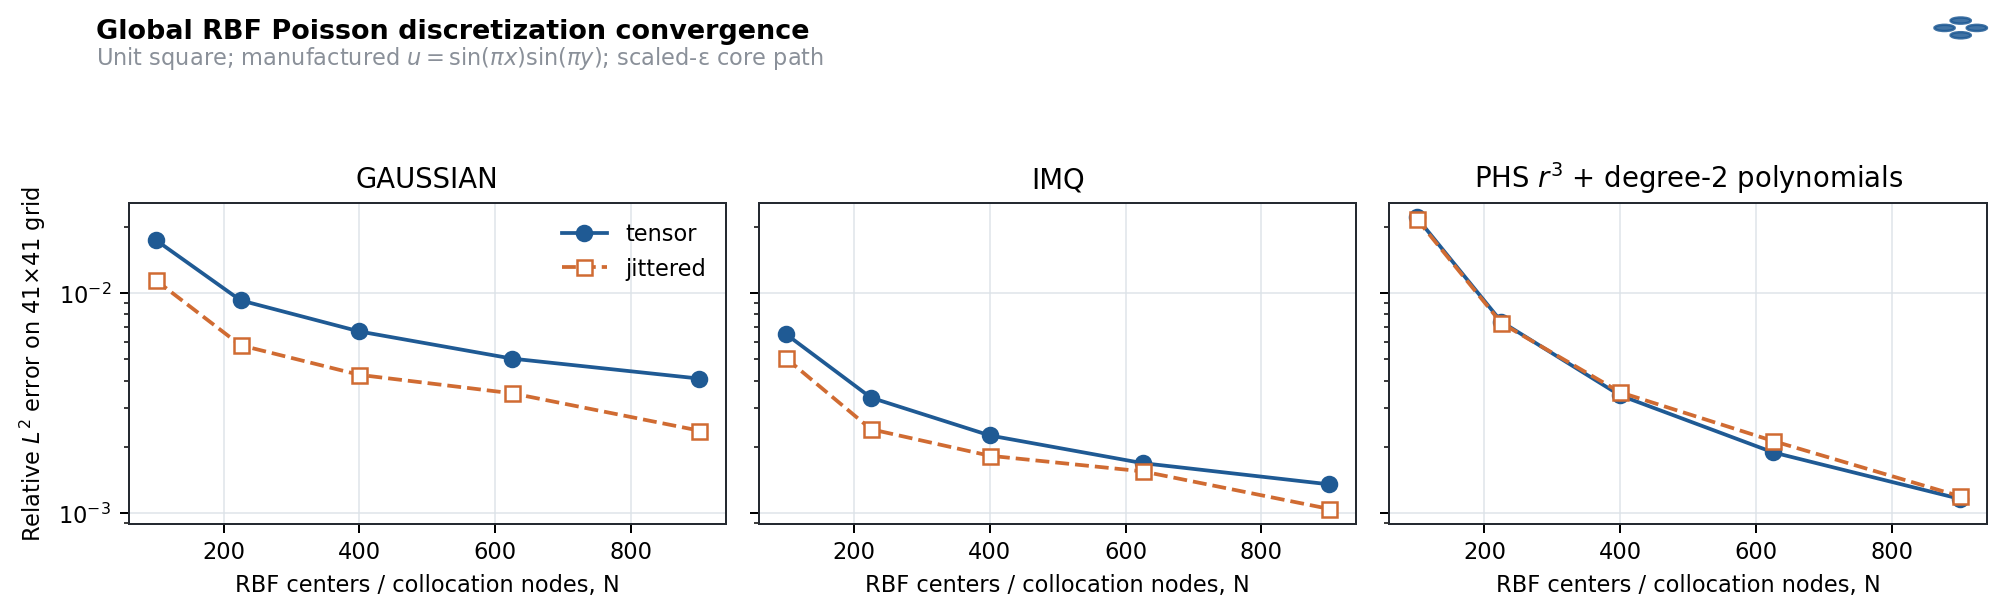
\includegraphics[width=\textwidth]{figures/discretization_convergence.png}
  \caption{Relative evaluation-grid error along the resolved global-collocation paths. The shape parameters scale with grid size so this figure validates the discretization rather than claiming fixed-shape spectral convergence.}
  \label{fig:discretization}
\end{figure}

\begin{table}[H]
\centering
\caption{Discretization error and conditioning at the endpoints of the resolved path}
\label{tab:discretization}
\small
\begin{tabularx}{\textwidth}{l l r r r}
\toprule
Kernel & Nodes & Error at $N=100$ & Error at $N=900$ & $\kappa_2(A)$ at $N=900$ \\
\midrule
Gaussian & tensor & $1.74\times10^{-2}$ & $4.08\times10^{-3}$ & $2.13\times10^{11}$ \\
Gaussian & jittered & $1.14\times10^{-2}$ & $2.37\times10^{-3}$ & $4.20\times10^{9}$ \\
IMQ & tensor & $6.49\times10^{-3}$ & $1.35\times10^{-3}$ & $5.77\times10^{9}$ \\
IMQ & jittered & $5.04\times10^{-3}$ & $1.04\times10^{-3}$ & $3.72\times10^{9}$ \\
PHS $r^3$ with polynomials & tensor & $2.20\times10^{-2}$ & $1.16\times10^{-3}$ & $4.00\times10^{8}$ \\
PHS $r^3$ with polynomials & jittered & $2.17\times10^{-2}$ & $1.19\times10^{-3}$ & $4.02\times10^{8}$ \\
\bottomrule
\end{tabularx}
\end{table}

The flat Gaussian regime exposes the limit of this formulation. At $N=225$ and $\epsilon=2$, the grid error is $1.73\times10^{-7}$ while $\kappa_2(A)=4.40\times10^{19}$. At $N=400$, the corresponding condition number is $1.38\times10^{20}$. A small manufactured-solution error does not make arbitrary inverse actions trustworthy. Those rows were retained only as sensitivity evidence. Stable-basis methods such as RBF-QR are the appropriate numerical tool for the flat limit \cite{fornberg2011}.

The first dense benchmark showed that FP64 pivoted LU is the fastest and most reliable method at moderate $N$. FP32 pivoted LU is the strongest reusable iterative action. A later three-way comparison added the local LS-ACBF method without changing the 27 fixed $N=225$ Gaussian systems. This changed the interpretation from FP32 LU being the only credible baseline to FP32 LU being the best primary baseline while LS-ACBF is a valid RBF-specific comparator. Figure~\ref{fig:classical} and Table~\ref{tab:classical} show why.

\begin{figure}[H]
  \centering
  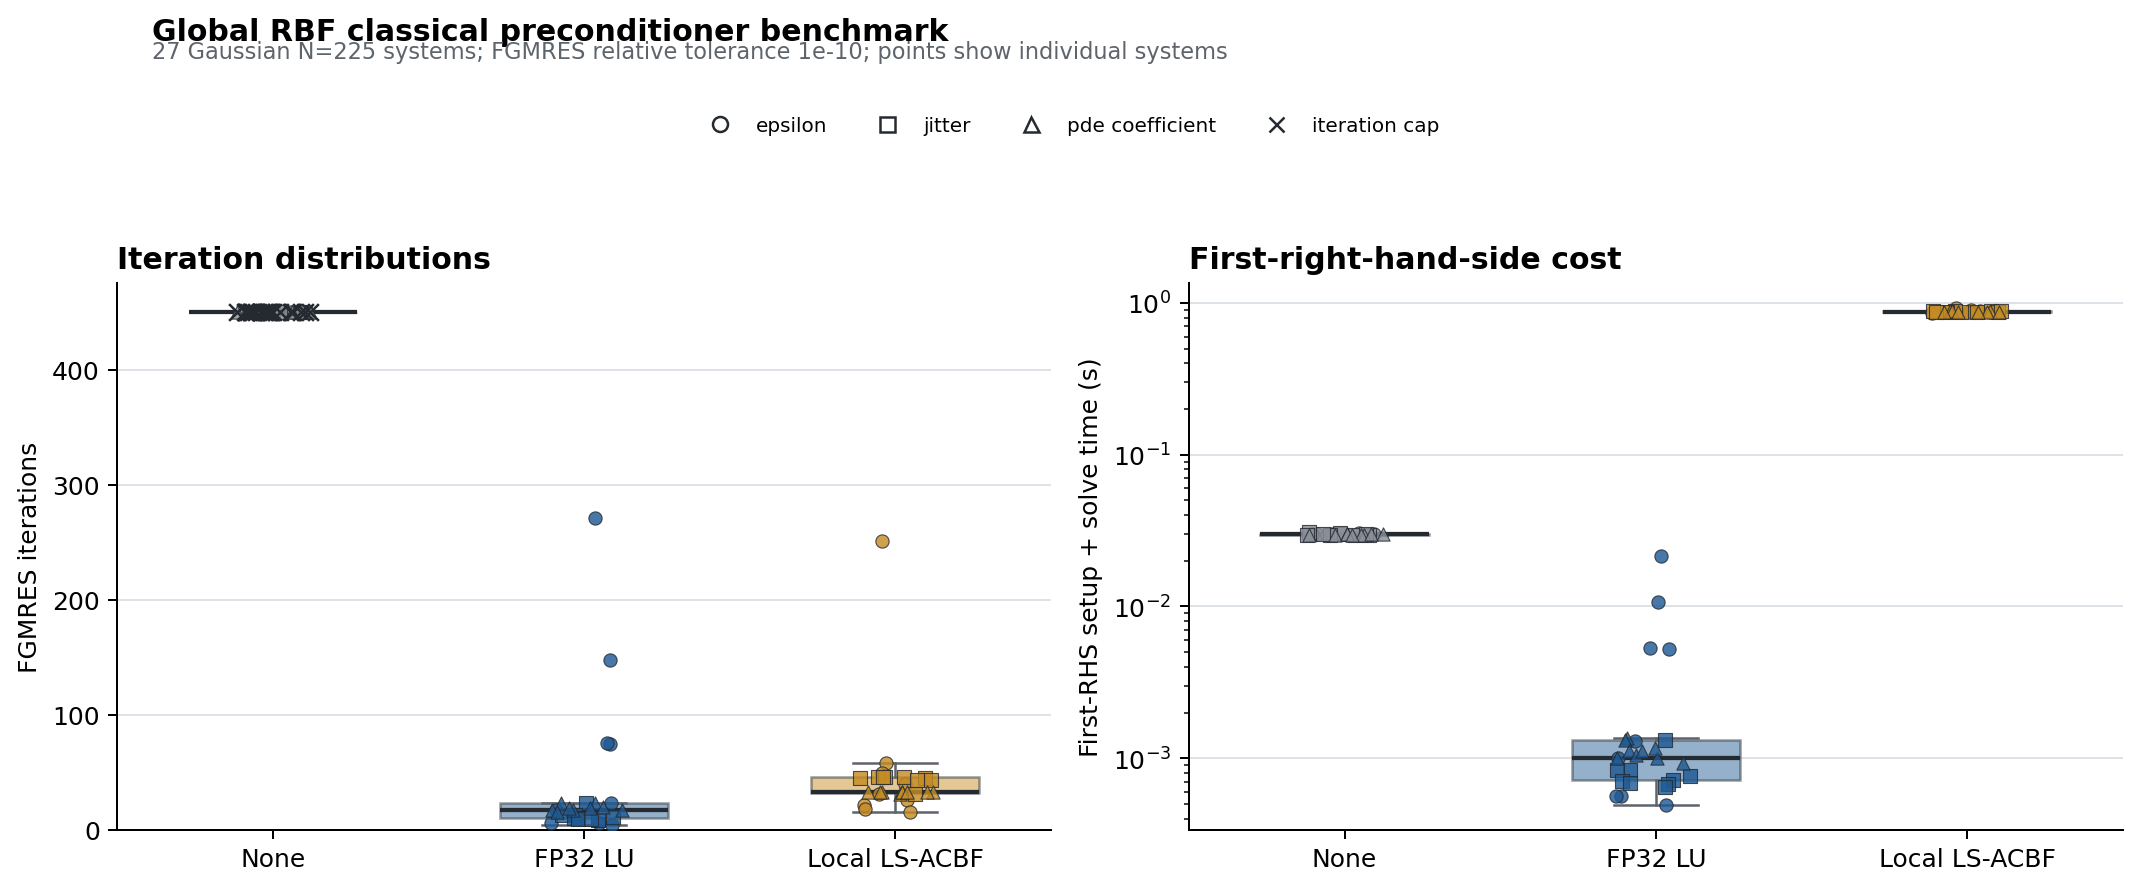
\includegraphics[width=0.94\textwidth]{figures/classical_preconditioner_comparison.png}
  \caption{Iterations and first-right-hand-side cost on the 27-system $N=225$ family. Crosses denote capped nonconverged runs.}
  \label{fig:classical}
\end{figure}

\begin{table}[H]
\centering
\caption{Three classical baselines on the fixed $N=225$ Gaussian family}
\label{tab:classical}
\small
\begin{tabularx}{\textwidth}{X r r r r r}
\toprule
Method & Converged & Median iterations & Setup & Solve & Memory \\
\midrule
None & 0/27 & 450 cap & 0 & 29.81 ms & 0 \\
FP32 pivoted LU & 27/27 & 17 & 0.320 ms & 0.690 ms & 0.203 MB \\
LS-ACBF, $k=161$ & 27/27 & 33 & 874.53 ms & 1.920 ms & 0.436 MB \\
\bottomrule
\end{tabularx}
\end{table}

LS-ACBF beat FP32 LU in both iterations and online time for the four flattest systems from $\epsilon=5.00$ to $5.75$. Its setup moved estimated break-even to 111 to 1062 repeated right-hand sides. At $N=225$, the robust support uses 161 of 225 equations per row, so locality is weak. FP32 LU therefore remains the primary $M$ for the compact parameter families. LS-ACBF becomes useful later because it creates a convergent but nontrivial $N=400$ benchmark.

The large-size scaling experiment kept $\epsilon=0.4\sqrt N$, so $\epsilon h$ stayed near 0.4. From $N=900$ to $10{,}000$, matrix storage grew from 6.48 MB to 800 MB and the estimated condition number grew from $2.13\times10^{11}$ to $1.27\times10^{13}$. None, Jacobi, LS-ACBF with $k=49$, and FP32 LU all missed the $10^{-10}$ target within 1000 steps on the measured rows. The iteration counts are therefore censored and cannot rank methods. At $N=4900$, a harmonic-Ritz recycle follow-up with right Jacobi also left every rank at the 1000-step cap and increased the terminal residual from $4.97\times10^{-5}$ to as much as $1.50\times10^{-4}$. These cases diagnose native-basis scaling failure rather than useful recycling difficulty.

\section{Difficult spaces depend on the solver integration}

The first structural study found that $d(r)$ is compressible on selected systems but not uniformly low rank. Capturing 99\% of snapshot energy required $q/N$ from 0.005 to 0.08. Reaching a median held-out projection error below 1\% required $q/N$ from 0.02 to 0.107. Energy concentration alone was therefore optimistic.

An early system-own oracle using the smallest right singular vectors of $A$ with a residual-complement Petrov correction produced a striking result. At $q=32$, the median iteration ratio was 0.250 and all 20 system and right-hand-side comparisons improved. The setup cost was roughly 28 classical solves, and the gain appeared abruptly between $q=24$ and $q=32$. A transfer study then showed that the corresponding subspace map was geometrically systematic. At $q=32$, Spearman correlation between parameter distance and normalized projector distance was 0.960 for $\epsilon$, 0.977 for jitter, and 0.821 for $\beta$. Within-system perturbation distances were about $10^{-8}$ while adjacent-system distances ranged from roughly $8\times10^{-3}$ to $7\times10^{-2}$.

That geometric result did not imply reusable solver benefit. Nearby $q=32$ spaces required 6.63, 2.71, and 27.88 times the own-oracle iterations for the $\epsilon$, jitter, and PDE families. The geometry was measured through principal angles and basis-invariant projector distances \cite{bjorck1973,edelman1998}. Grassmann interpolation \cite{amsallem2008} was useful only for the PDE path, where it needed a median eight iterations compared with four for the own oracle and 111.5 for one-sided reuse.

\begin{figure}[H]
  \centering
  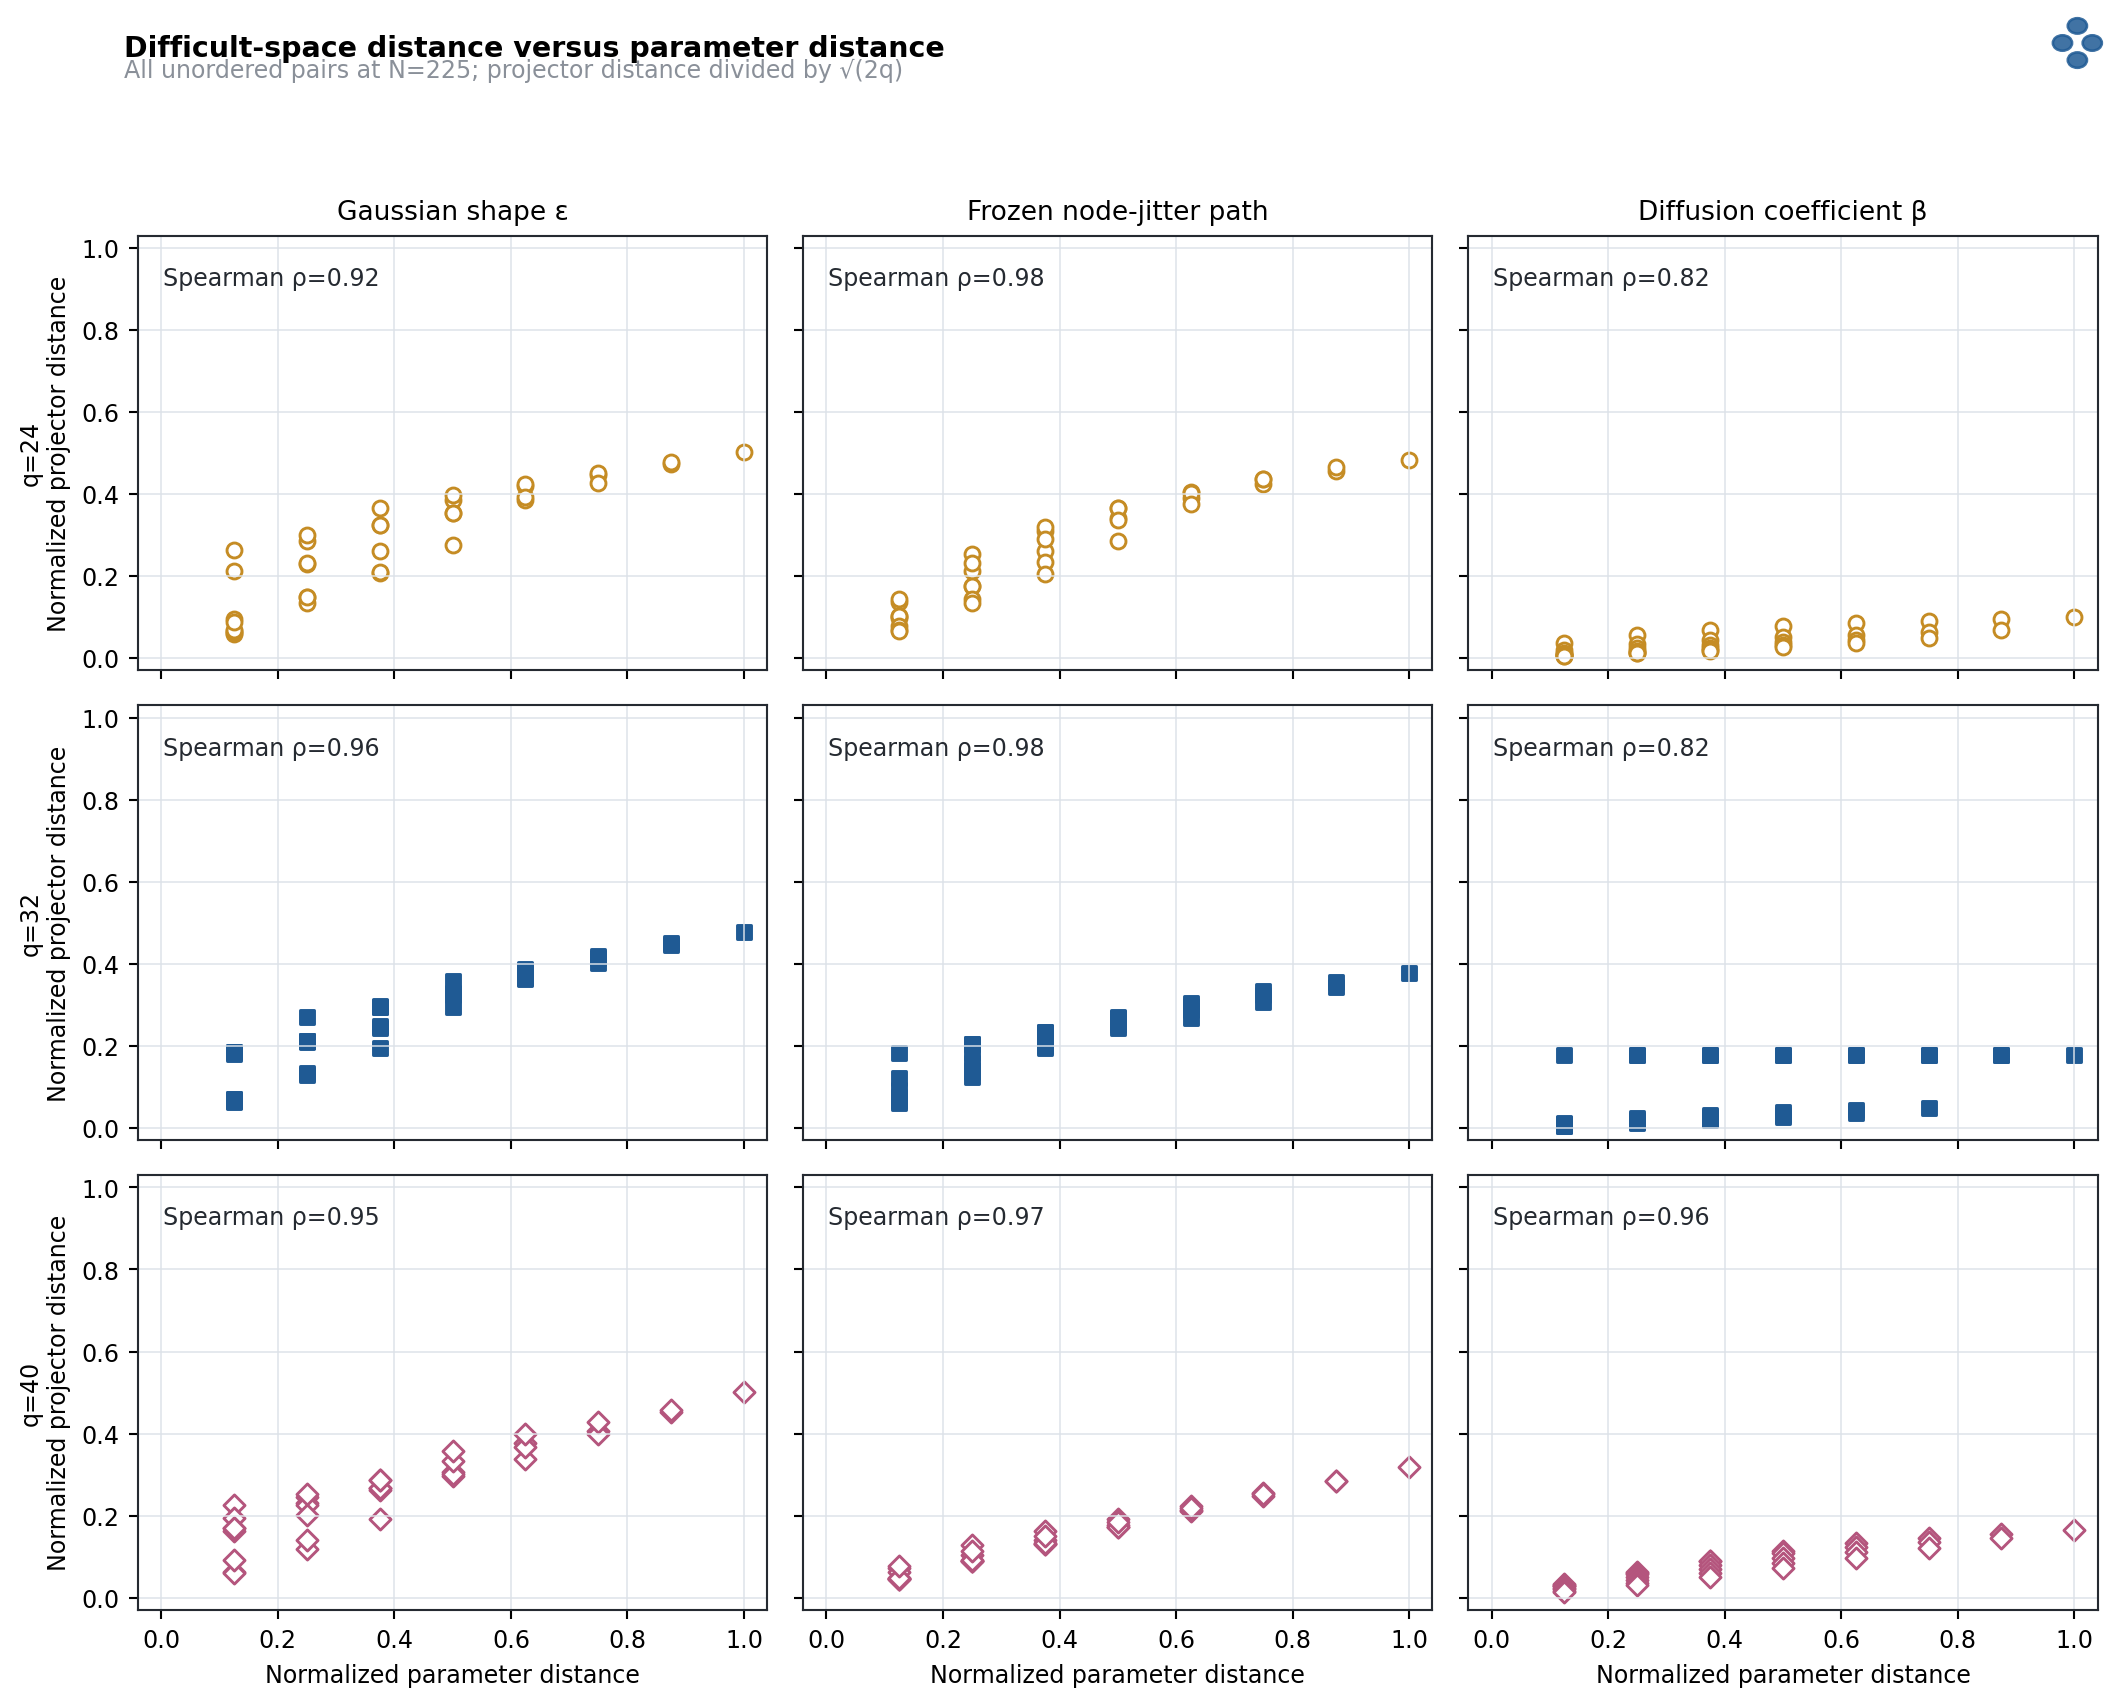
\includegraphics[width=0.90\textwidth]{figures/subspace_distance_vs_parameter_distance.png}
  \caption{The $N=225$ smallest-singular-vector family is systematically ordered by parameter distance in an average Grassmann metric.}
  \label{fig:stage2}
\end{figure}

\begin{figure}[H]
  \centering
  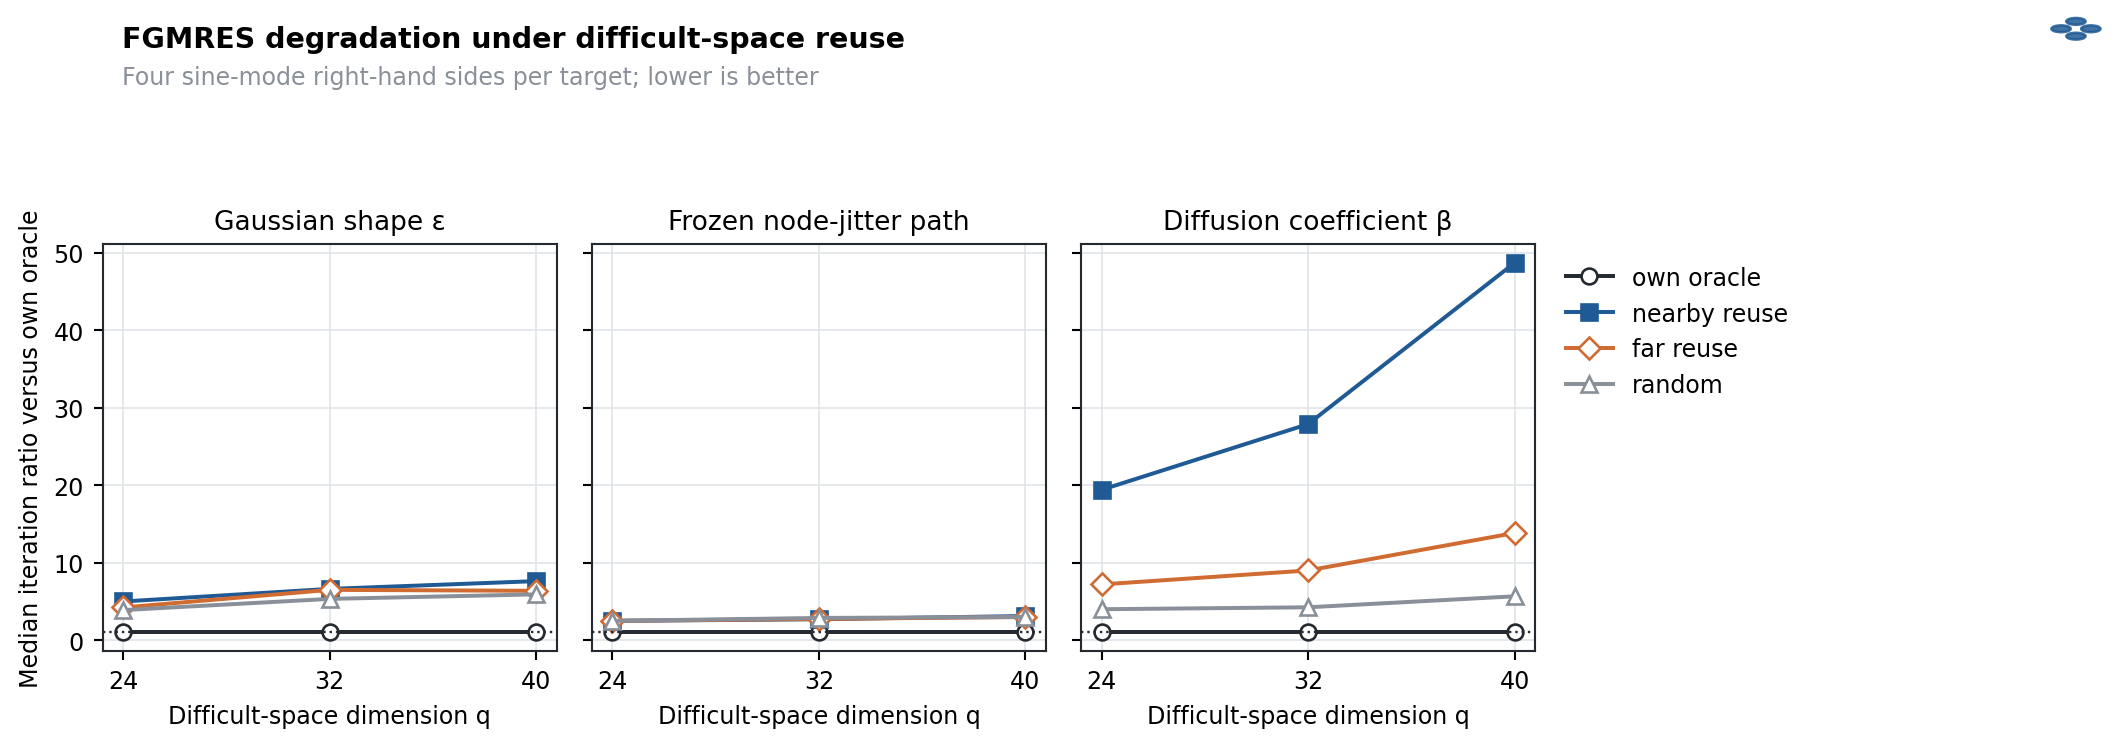
\includegraphics[width=0.96\textwidth]{figures/reuse_solver_degradation.png}
  \caption{Geometric regularity does not preserve own-oracle acceleration. The coarse solver is sensitive to particular directions within the nearby spaces.}
  \label{fig:reuse}
\end{figure}

The next experiments changed one point at a time to remove confounding. First, three target definitions were compared under the same additive correction. Dominant right singular vectors of $S_L$ were least harmful, with a median ratio of 1.013 at $q=8$, while small singular vectors of $B_L$ and late residual POD were worse. No candidate reduced aggregate median iterations or time. Second, additive Galerkin, QR or SVD residual minimization, and standard deflation were compared using the same exact $S_L$ space. Standard deflation was strongest, but its aggregate median ratio remained 1.000.

The final fair comparison fixed standard deflation and tested small right singular vectors of $A$, dominant right singular vectors of $S_L$, and small right singular vectors of $B_L$. The dominant $S_L$ space at $q=16$ was the robustness winner with 108 of 108 converged solves and median ratio 1.000. Small singular vectors of $A$ were unusable under this integration, with median ratios above 8.8 and fewer than half of the solves converging. This does not contradict the earlier $A$-small oracle. It shows that a target space and its coarse action form one algorithmic object.

\begin{figure}[H]
  \centering
  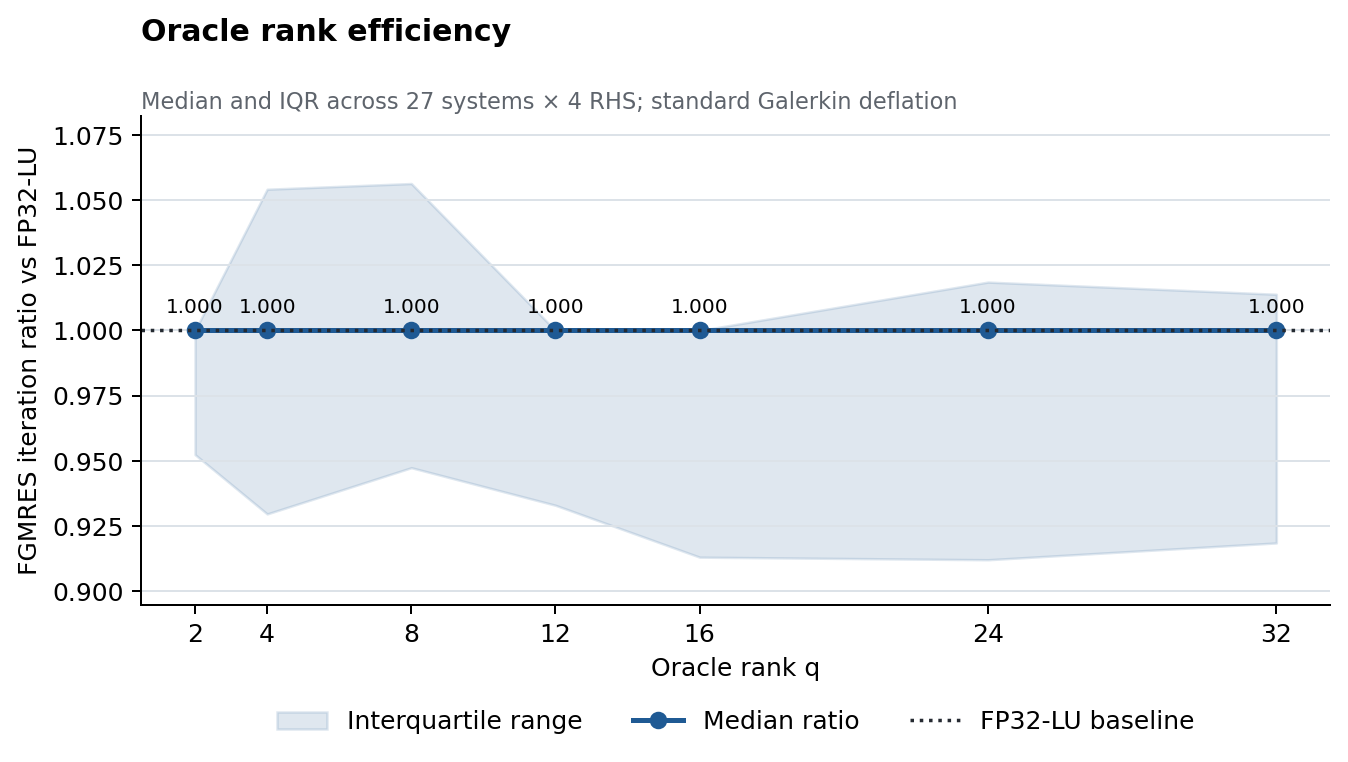
\includegraphics[width=0.78\textwidth]{figures/rank_efficiency.png}
  \caption{Rank efficiency of the dominant $S_L$ target under standard deflation. Every tested median iteration ratio is one, so increasing rank does not establish a useful low-dimensional correction.}
  \label{fig:rank}
\end{figure}

Baseline FGMRES dynamics gave a more direct diagnostic. On the 27-system $N=225$ suite, late exact-error POD at $q=4$ was the most robust same-trajectory target on slow solves. Its median ratio was 0.783 in the slowest quartile, with 26 of 29 converged cases. Harmonic Ritz and unresolved-correction POD sometimes reduced nominal iterations more strongly, but frequent nonconvergence made those reductions unreliable. This result is deliberately described as an on-trajectory oracle. It does not show operator-level reuse.

\begin{table}[H]
\centering
\caption{How the target recommendation changed when the comparison became stricter}
\label{tab:targettrail}
\footnotesize
\begin{tabularx}{\textwidth}{Y Y p{0.17\textwidth} Y}
\toprule
Population and integration & Space & Key result & Interpretation \\
\midrule
Five systems with residual-complement Petrov action & Small right singular vectors of $A$, $q=32$ & Median ratio 0.250 & Strong system-own upper bound with expensive SVD \\
Four $N=225$ systems with additive action & Dominant right singular vectors of $S_L$, $q=8$ & Median ratio 1.013 & Best of three targets, but no aggregate gain \\
Twenty-seven $N=225$ systems with standard deflation & Dominant right singular vectors of $S_L$, $q=16$ & Median ratio 1.000, 108/108 converged & Robustness winner only \\
Slowest trajectory quartile with standard deflation & Late exact-error POD, $q=4$ & Median ratio 0.783, 26/29 converged & Same-trajectory diagnostic, not a reusable target \\
\bottomrule
\end{tabularx}
\end{table}

The combined conclusion from these experiments is that no matrix-only spectral definition is uniformly solver relevant. Low rank is not enough, average projector distance is not enough, and a favorable oracle under one correction cannot be transferred to another integration without retesting.

\section{A hard recycle benchmark reveals target-specific acceleration}

The broad $N=225$ family was often too easy after FP32 LU, while the native-basis cases from $N=900$ upward did not converge. A targeted transition search kept the same Gaussian Poisson formulation and tested $N=400$, 625, and 900 with Jacobi, FP32 LU, and LS-ACBF. Only one case met both requirements of true convergence and 100 to 800 iterations. It uses $N=400$, $\epsilon=8$, tensor nodes, and LS-ACBF with $k=81$. Baseline FGMRES required 486 iterations and reached $9.95\times10^{-11}$.

The next experiment added only an exact harmonic-Ritz recycle space extracted from the converged baseline trajectory. The projected-Arnoldi integration and all solver settings remained fixed. Table~\ref{tab:recycle} shows a clear same-system effect. The $q=16$ space reduced iterations from 486 to 352, while the matched random space needed 474.

\begin{table}[H]
\centering
\caption{Exact harmonic-Ritz recycling on the validated $N=400$ benchmark}
\label{tab:recycle}
\small
\begin{tabularx}{\textwidth}{X r r r r}
\toprule
Method & Iterations & True relative residual & Solve time & Iteration ratio \\
\midrule
Baseline LS-ACBF FGMRES & 486 & $9.95\times10^{-11}$ & 0.0515 s & 1.000 \\
Harmonic Ritz, $q=4$ & 370 & $9.60\times10^{-11}$ & 0.0392 s & 0.761 \\
Random, $q=4$ & 479 & $9.86\times10^{-11}$ & 0.0519 s & 0.986 \\
Harmonic Ritz, $q=8$ & 381 & $9.55\times10^{-11}$ & 0.0411 s & 0.784 \\
Random, $q=8$ & 500 & $9.48\times10^{-11}$ & 0.0555 s & 1.029 \\
Harmonic Ritz, $q=16$ & 352 & $9.88\times10^{-11}$ & 0.0377 s & 0.724 \\
Random, $q=16$ & 474 & $9.92\times10^{-11}$ & 0.0514 s & 0.975 \\
\bottomrule
\end{tabularx}
\end{table}

The augmentation identities were accurate. At $q=16$ they satisfy

\begin{equation*}
\norm{AU-C}_F=1.04\times10^{-10},
\qquad
\norm{C\trans C-I}_F=1.55\times10^{-15}.
\end{equation*}

The baseline extraction cost was excluded from the online solve. This is the strongest evidence in the project that a low-dimensional Krylov-derived space can matter when the classical baseline is convergent but not trivial.

The transfer experiment then changed only $\epsilon$. Each source space was mapped to the target operator by recomputing $A_tU=C$ and renormalizing. Across eight directed adjacent transfers from $\epsilon=7.6$ to $8.4$, the median transfer-to-baseline ratio was 0.989. None met the strong criterion of 0.85, only two fell in the weakly useful range, and every transfer at distance at least 0.4 was slower than baseline. Figure~\ref{fig:heatmap} shows the full directional pattern.

\begin{figure}[H]
  \centering
  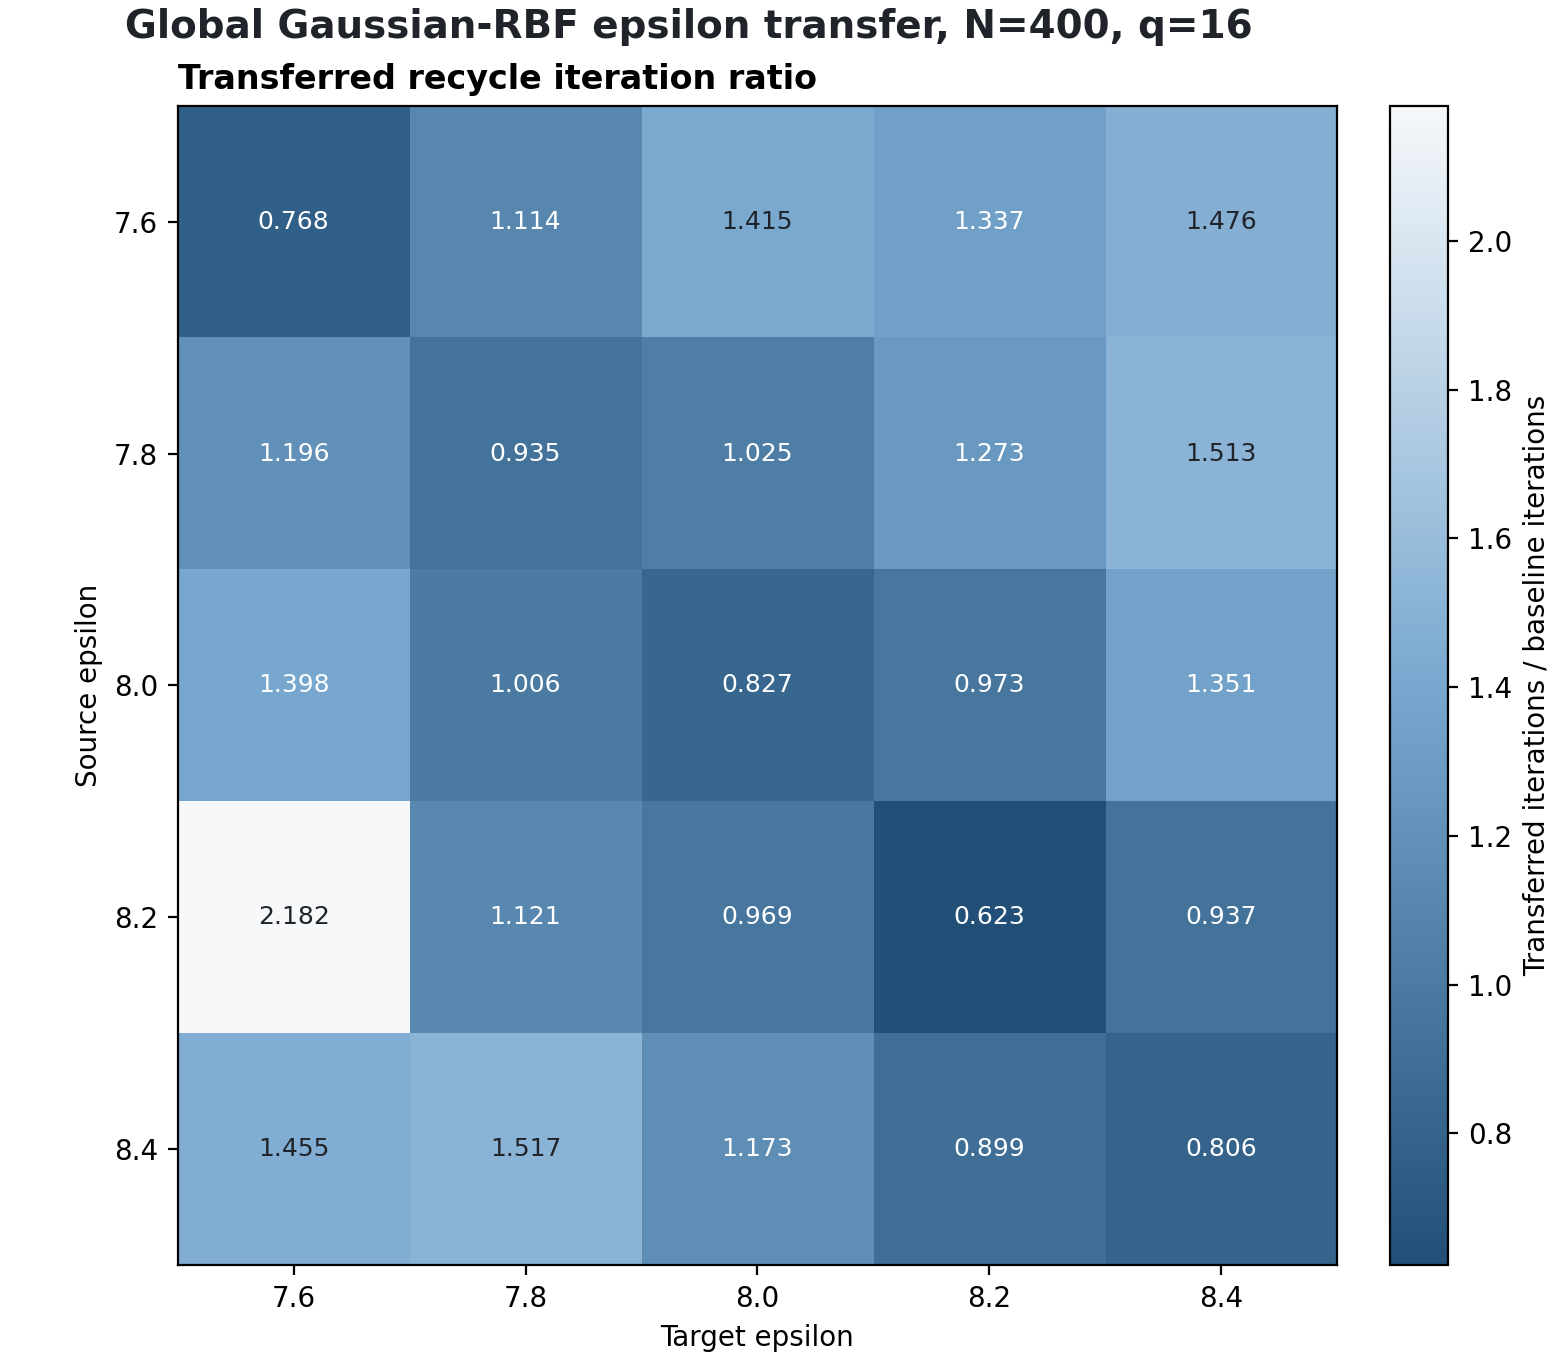
\includegraphics[width=0.76\textwidth]{figures/epsilon_transfer_heatmap.png}
  \caption{Transferred harmonic-Ritz iteration ratio. Diagonal cells are self-oracles. Off-diagonal performance degrades rapidly and is direction dependent.}
  \label{fig:heatmap}
\end{figure}

Adjacent spaces had median largest principal angle 88.2 degrees and median projector distance 4.03, where the maximum for rank 16 is $\sqrt{32}$. Geometry correlated with degradation only moderately because geometric distance is symmetric while solver behavior is directional. The target-specific oracles remained useful, with ratios from 0.623 to 0.935. The information exists but does not persist across nearby systems.

The cluster diagnostic tested whether rank 16 cut through nearly tied harmonic Ritz values. Relative adjacent gaps below 5\% defined a cluster. The complete common ranks were 16 for the 7.8 and 8.0 pair, 20 for the 8.0 and 8.2 pair, and 17 for the 8.2 and 8.4 pair. Figure~\ref{fig:clusters} shows the first 30 Ritz magnitudes and the local gaps.

\begin{figure}[H]
  \centering
  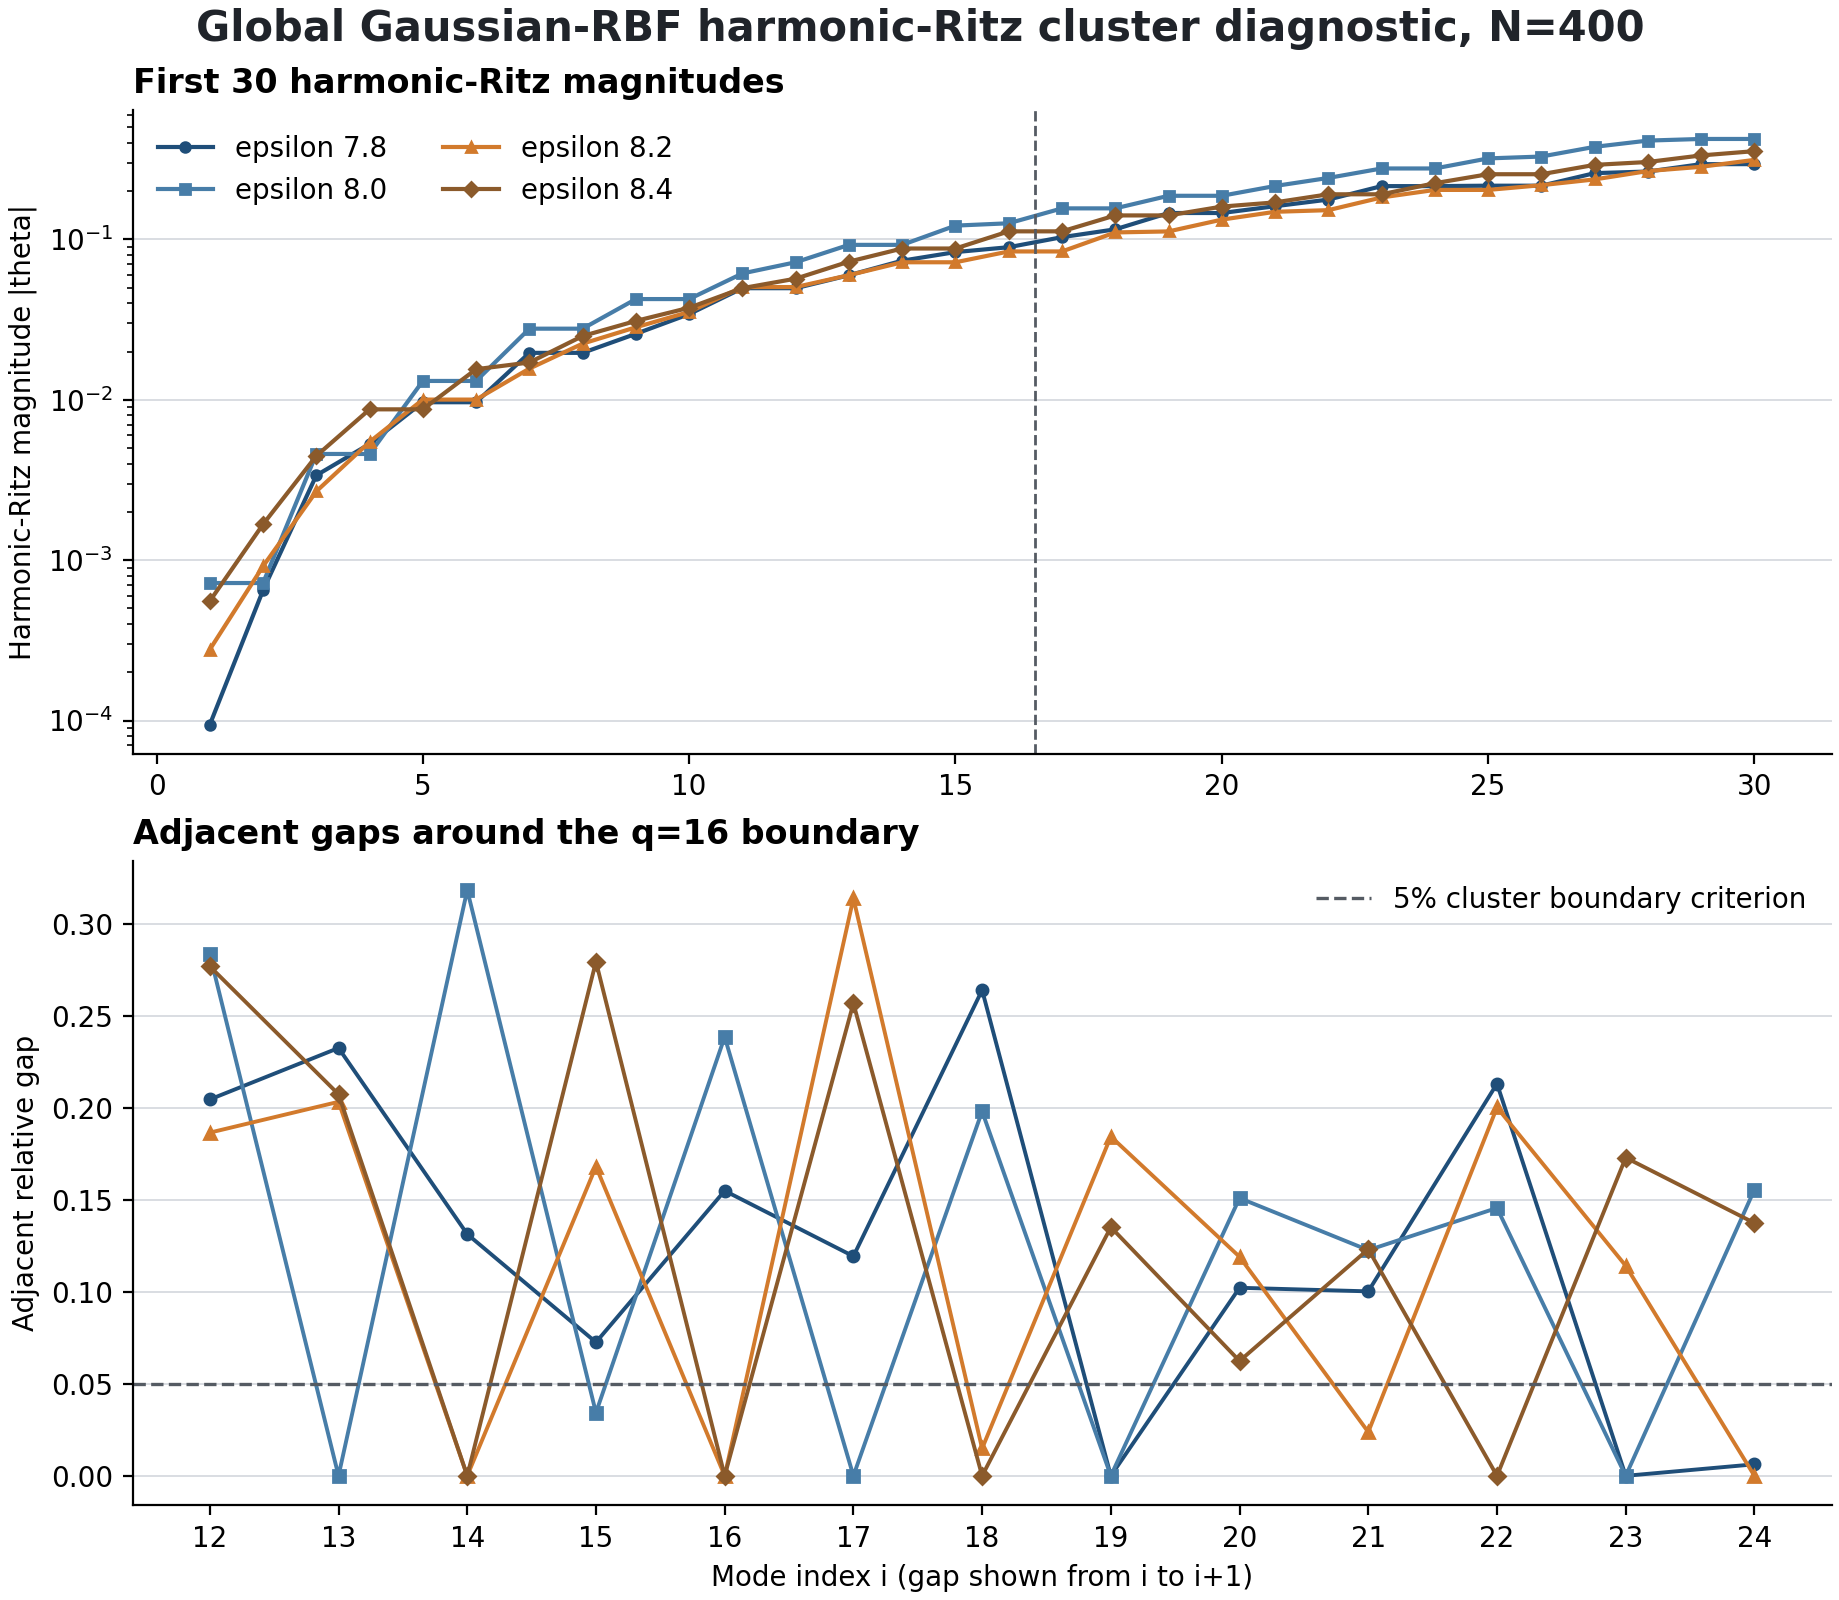
\includegraphics[width=0.88\textwidth]{figures/harmonic_ritz_spectra_and_gaps.png}
  \caption{Harmonic-Ritz magnitudes and adjacent relative gaps near the rank-16 boundary. Cluster completion changes the rank but does not create a stable transferable prefix.}
  \label{fig:clusters}
\end{figure}

Cluster-aware transfer had median ratio 0.974 compared with 0.971 for fixed $q=16$. Only one of six directed pairs reached 0.90, and normalized projector distance worsened from 0.681 to 0.699. Own-system spaces remained effective at $q=20$ and $q=24$. The failure is therefore not caused mainly by an artificial fixed-rank cut. The current harmonic-Ritz prefix is a useful self-oracle and a poor transferable target.

\section{The learning gate remains closed}

An offline data set was prepared before later experiments fully exposed the target weakness. It fixed $N=225$, tensor nodes, the Gaussian kernel, and the variable-diffusion PDE. Only $\epsilon$ and $\beta$ varied. Each of 113 parameter pairs stored the dominant $q=8$ right singular vectors of $S_L$, the classical and oracle iteration counts for four diagnostic right-hand sides, and a coefficient representation in a shared training basis.

The shared basis $W$ was computed from concatenated training spaces. The smallest prefix reaching 99.9\% training energy had $p=158$, which is 70.2\% of the full coefficient dimension. Median projector reconstruction error was 0.119 on training, 0.210 on validation, and 0.190 on test. The median paired oracle iteration ratio was 1.018 on training, 1.000 on validation, and 1.050 on test. Only 18 of 113 systems had verified median acceleration with full convergence. The data set is leakage-free and numerically valid, but the target is neither compact nor solver-useful enough to support the planned MLP.

Residual-history POD was the final alternative target diagnostic. True residuals were saved every 10 iterations and at every restart boundary for $\epsilon=7.8$, 8.0, 8.2, and 8.4 on the $N=400$ LS-ACBF benchmark family. Each snapshot was normalized before SVD. Rank four captured 52\% to 67\% of energy and rank eight captured 75\% to 79\%. At rank 16 the energy reached 91\% to 98\%, but rank 16 already consumed 23\% to 76\% of the available snapshots.

\begin{figure}[H]
  \centering
  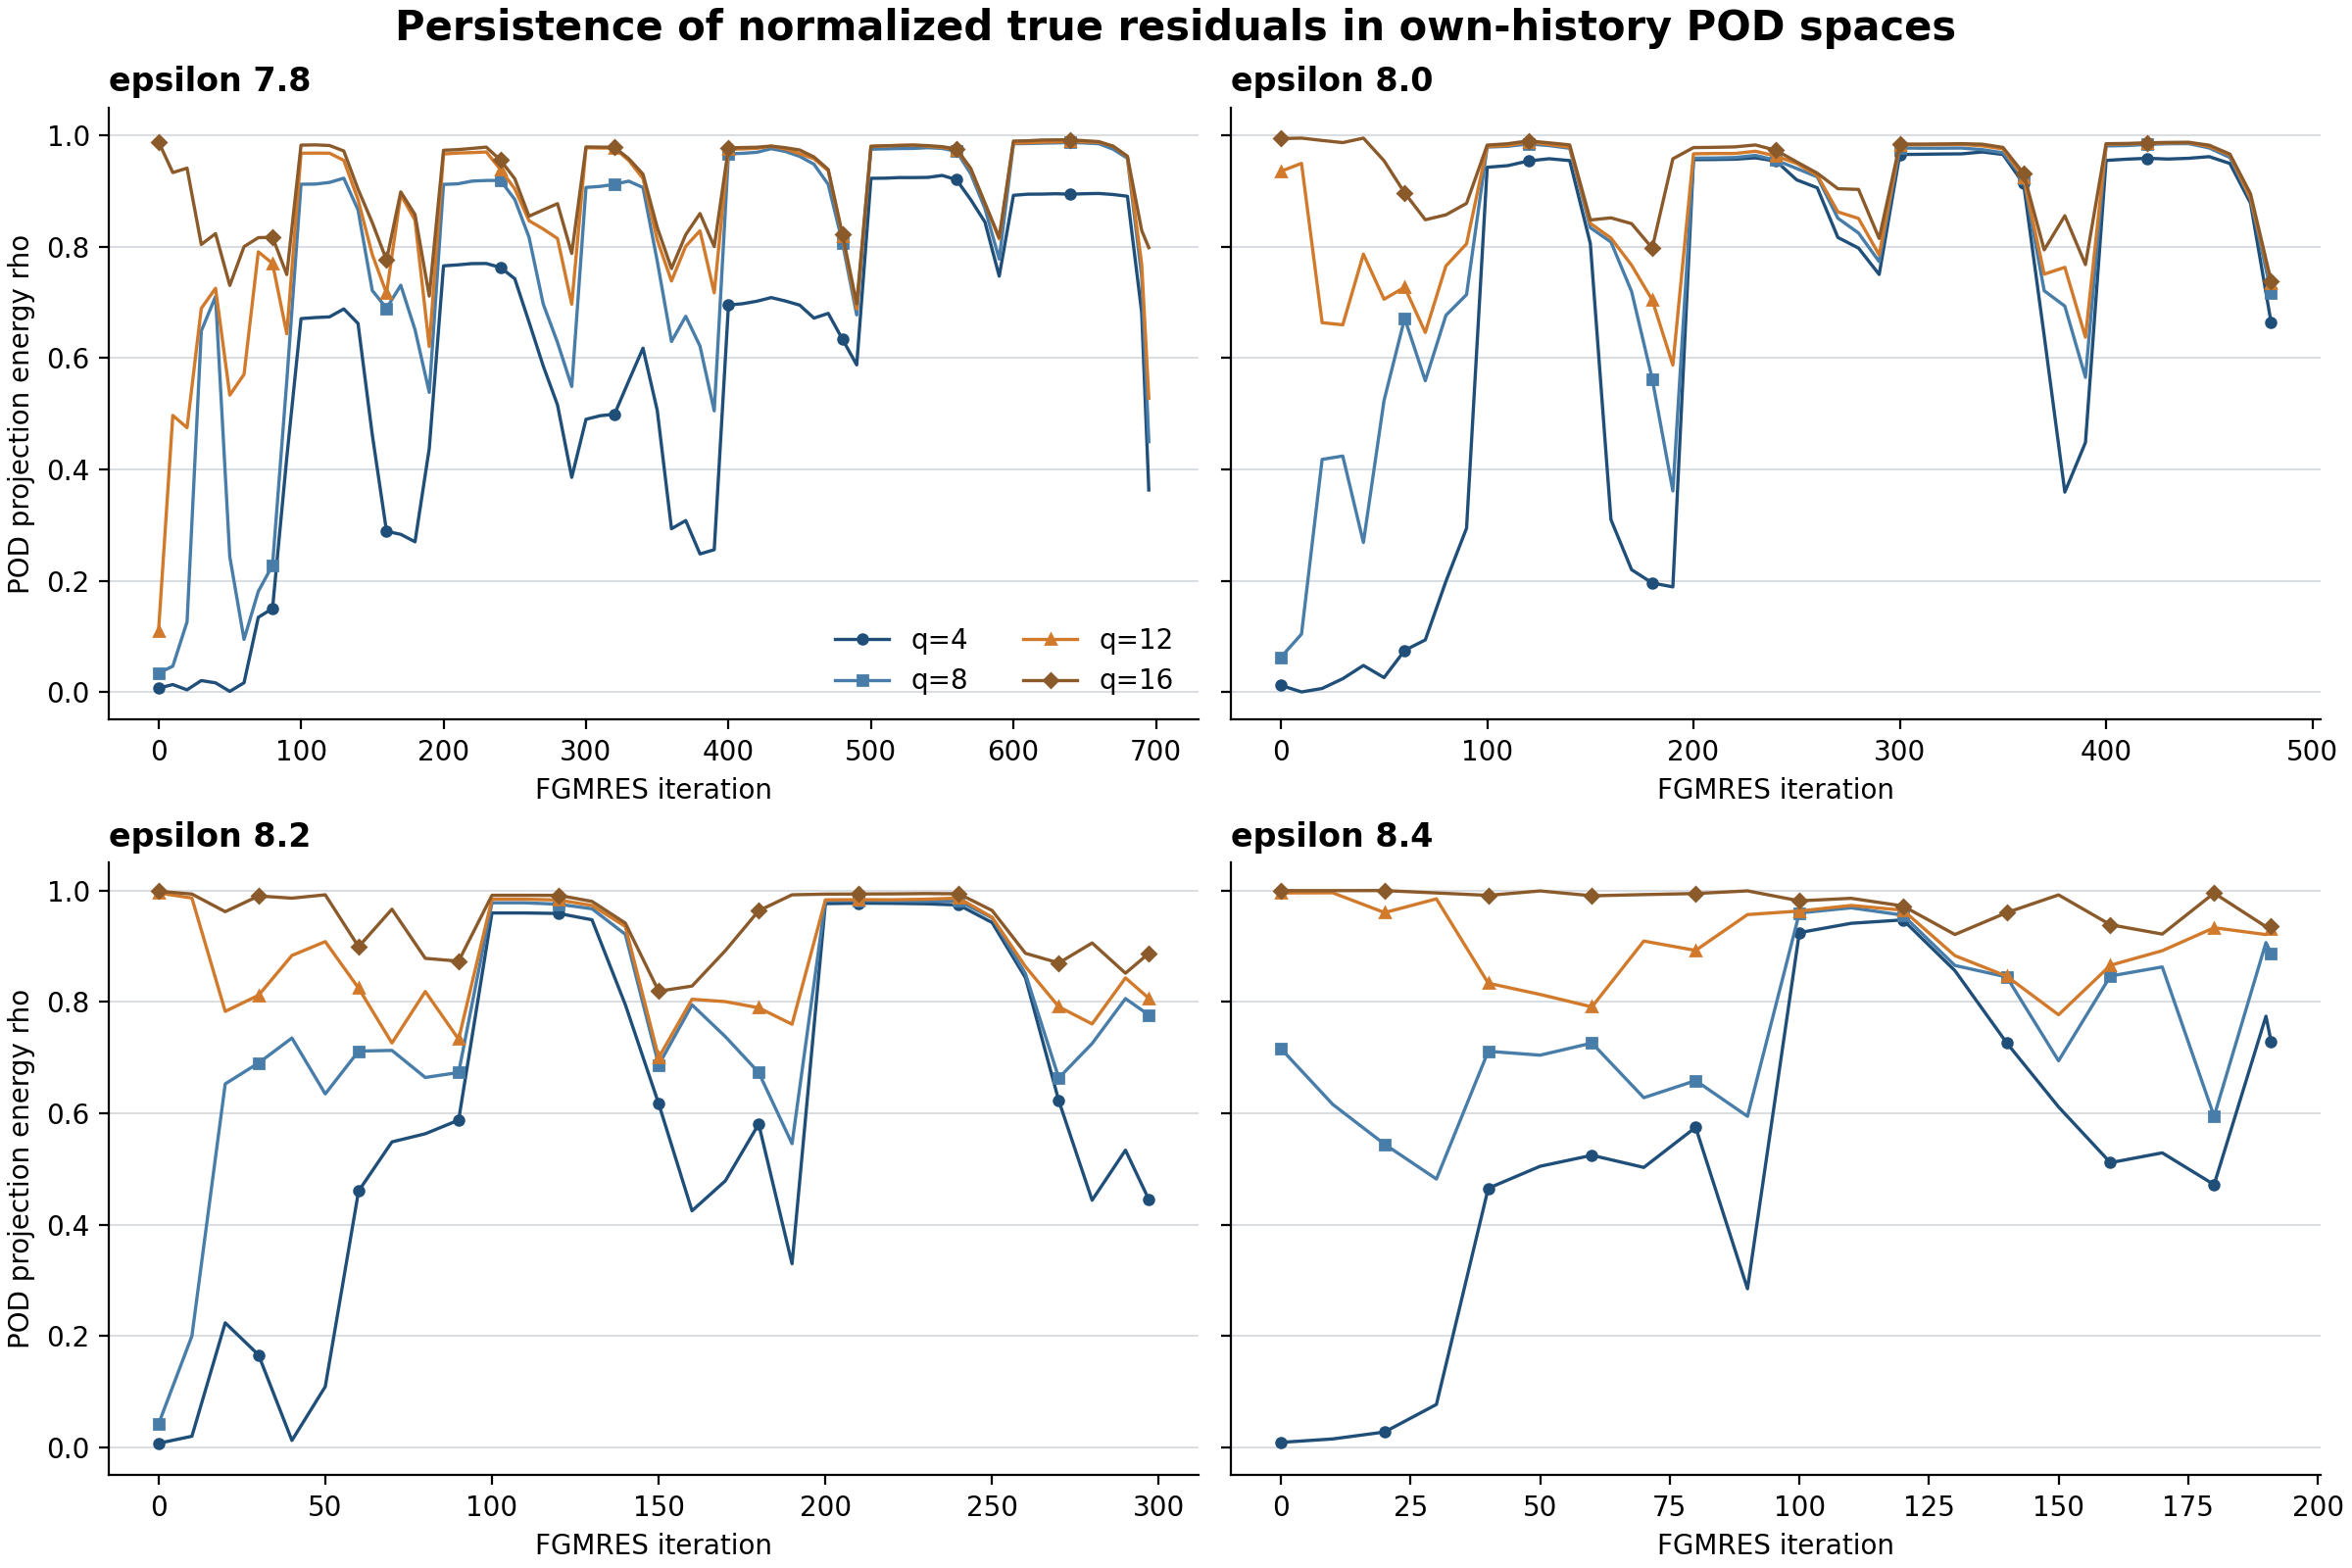
\includegraphics[width=0.92\textwidth]{figures/residual_pod_persistence.png}
  \caption{Projection energy of normalized true residuals onto their own-history POD spaces. Restart-scale oscillation dominates and late concentration is not systematic across epsilon.}
  \label{fig:residualpod}
\end{figure}

Late concentration increased consistently only at $\epsilon=7.8$. At $\epsilon=8.2$, the late-quartile median minus the previous-quartile median was negative for every tested rank. At $\epsilon=8.4$, every late-half slope was negative. Cross-epsilon geometry was also worse than harmonic Ritz. At $q=16$, residual POD had median normalized projector distance 0.820 compared with 0.681 for harmonic Ritz, and the largest principal angles were near 90 degrees. Because the target failed the structural gate even on the trajectories used to construct it, no lifting, recycle solve, transfer test, or neural model was run.

The combined learning conclusion is negative but informative. The project has not failed because neural prediction was inaccurate. Neural prediction was never reached because the numerical target did not satisfy its prerequisites. This avoids training a model to approximate a space that is expensive, high dimensional, unstable, or ineffective under the actual solver integration.

\section{Current problem and next directions}

The current problem is a mismatch between strong local oracle information and weak cross-system persistence. On the validated $N=400$ case, a rank-16 harmonic-Ritz space reduces iterations by 27.6\%. Across nearby $\epsilon$, nearly the same construction gives a median ratio near one. Small average subspace distance is also insufficient. In the $N=225$ PDE family, a normalized projector distance below 0.01 can still accompany severe reuse degradation. At larger $N$, the native Gaussian basis and available classical actions fail before recycling can be assessed cleanly.

The next work should improve the numerical object before improving the predictor:

\begin{enumerate}[label=\arabic*.]
  \item Replace or stabilize the native Gaussian basis in the flat and large-$N$ regimes. RBF-QR, localized bases, partition-of-unity formulations, hierarchical compression, or domain decomposition should be tested while preserving true-residual validation.
  \item Define a recycle target from solver action rather than an unweighted Euclidean projector. Candidate losses should measure the effect of omitted directions on projected Arnoldi or on $AM^{-1}$, with stability constraints on the reduced problem.
  \item Separate restart-cycle phase from persistent operator information. Residual POD should be revisited only with cycle-aligned snapshots or cross-right-hand-side validation.
  \item Track invariant blocks across parameters rather than fixed prefixes. Mode continuation should use principal-vector matching and preserve real two-dimensional blocks for complex conjugate pairs.
  \item Repeat the successful $N=400$ oracle on nearby PDE coefficients and on a second right-hand side. A target should retain at least a clear fraction of the self-oracle gain before interpolation or prediction is reconsidered.
  \item Keep deterministic interpolation as the learning baseline. The earlier PDE Grassmann result shows that a family-local interpolant can work, but it must be reproduced under the same validated recycle formulation.
\end{enumerate}

The final research position is therefore precise. Global RBF collocation contains exploitable low-dimensional solver information on individual systems. The present spaces do not vary regularly enough, or remain solver relevant enough, to make $\xi\mapsto V_{\mathrm{diff}}(\xi)$ a justified neural learning problem. Progress now depends on a better-conditioned formulation and a target whose transfer is defined by solver action.

\section*{Evidence and reproducibility}

This manuscript reconciles the primary reports for discretization and classical baselines, transferability of smallest-singular spaces, target and integration selection, rank efficiency, FGMRES trajectory oracles, large-size scaling, benchmark selection, exact $N=400$ recycling, epsilon transfer, Ritz-cluster diagnostics, residual-history POD, and the offline subspace data set. Later controlled results supersede quick-run summaries and earlier provisional target recommendations when they use a broader population or a common solver integration.

All reported convergence decisions use the original unpreconditioned $A$ and $b$. Independent validation reports recomputed the key residuals, ratios, projector metrics, Arnoldi and QR identities, and saved-basis orthogonality. The latest repository suite contains 69 passing tests. Raw evidence and scripts remain in the parent workspace under \texttt{results/}, \texttt{scripts/}, and \texttt{src/global\_rbf/}.

\begin{thebibliography}{9}

\bibitem{larsson2003}
E. Larsson and B. Fornberg.
\newblock A numerical study of some radial basis function based solution methods for elliptic PDEs.
\newblock \emph{Computers \& Mathematics with Applications}, 46, 2003.

\bibitem{fornberg2011}
B. Fornberg, E. Larsson, and N. Flyer.
\newblock Stable computations with Gaussian radial basis functions.
\newblock \emph{SIAM Journal on Scientific Computing}, 33(2), 2011.
\newblock \url{https://doi.org/10.1137/09076756X}.

\bibitem{saad1986}
Y. Saad and M. H. Schultz.
\newblock GMRES: A generalized minimal residual algorithm for solving nonsymmetric linear systems.
\newblock \emph{SIAM Journal on Scientific and Statistical Computing}, 7(3), 1986.
\newblock \url{https://doi.org/10.1137/0907058}.

\bibitem{morgan2002}
R. B. Morgan.
\newblock GMRES with deflated restarting.
\newblock \emph{SIAM Journal on Scientific Computing}.
\newblock \url{https://doi.org/10.1137/S0895479897321362}.

\bibitem{bjorck1973}
\AA. Bj\"orck and G. H. Golub.
\newblock Numerical methods for computing angles between linear subspaces.
\newblock \emph{Mathematics of Computation}, 27, 1973.
\newblock \url{https://doi.org/10.2307/2005662}.

\bibitem{edelman1998}
A. Edelman, T. A. Arias, and S. T. Smith.
\newblock The geometry of algorithms with orthogonality constraints.
\newblock \emph{SIAM Journal on Matrix Analysis and Applications}, 20(2), 1998.
\newblock \url{https://doi.org/10.1137/S0895479895290954}.

\bibitem{amsallem2008}
D. Amsallem and C. Farhat.
\newblock Interpolation method for adapting reduced-order models and application to aeroelasticity.
\newblock \emph{AIAA Journal}, 46(7), 2008.
\newblock \url{https://doi.org/10.2514/1.35374}.

\end{thebibliography}

\end{document}
